\section{Overview}
SHRINCS is designed in the way it can operate in two modes: \textbf{stateful} and \textbf{stateless}. Stateful mode is represented by the instance of Unbalanced XMSS (UXMSS) with a root public key \texttt{PK.sf}. An optimized variant of SPHINCS+ is used to support the stateless operating mode (which is represented by the public key \texttt{PK.sl}). The root public key is a hashed concatenation of (\texttt{PK.sf}, \texttt{PK.sl}), which is being converted to the Bitcoin address. 

During normal operation with intact state, the user generates signatures according to efficient stateful path. Each leaf of the UXMSS is represented by WOTS+C one time signature instance. UXMSS is right-skewed, which makes the first stateful signature (\texttt{q = 1}) the cheapest from the verification and size perspective and adds 16 bytes and one additional hash operation for each next stateful signature, up to \texttt{q = hsf}. The final signature (\texttt{q = hsf + 1}) has the same size and verification cost as \texttt{q = hsf}. A right-skewed UXMSS is a tree construction in which every internal node has a one-time signature leaf as its left child and a UXMSS subtree as its right child, yielding a recursively right-branching authentication tree (as shown on the Figure~1).

If the state is corrupted (or the limit for stateful operations is met), the scheme can continue operating with stateless mode. Stateless mode utilizes an optimized SPHINCS+ variant with WOTS+C signatures in regular XMSS trees on each layer in the hypertree and FORS+C for few-time signature scheme. The general construction of SHRINCS signature is presented on the Figure~1.
\begin{figure}[h!]
    \centering
    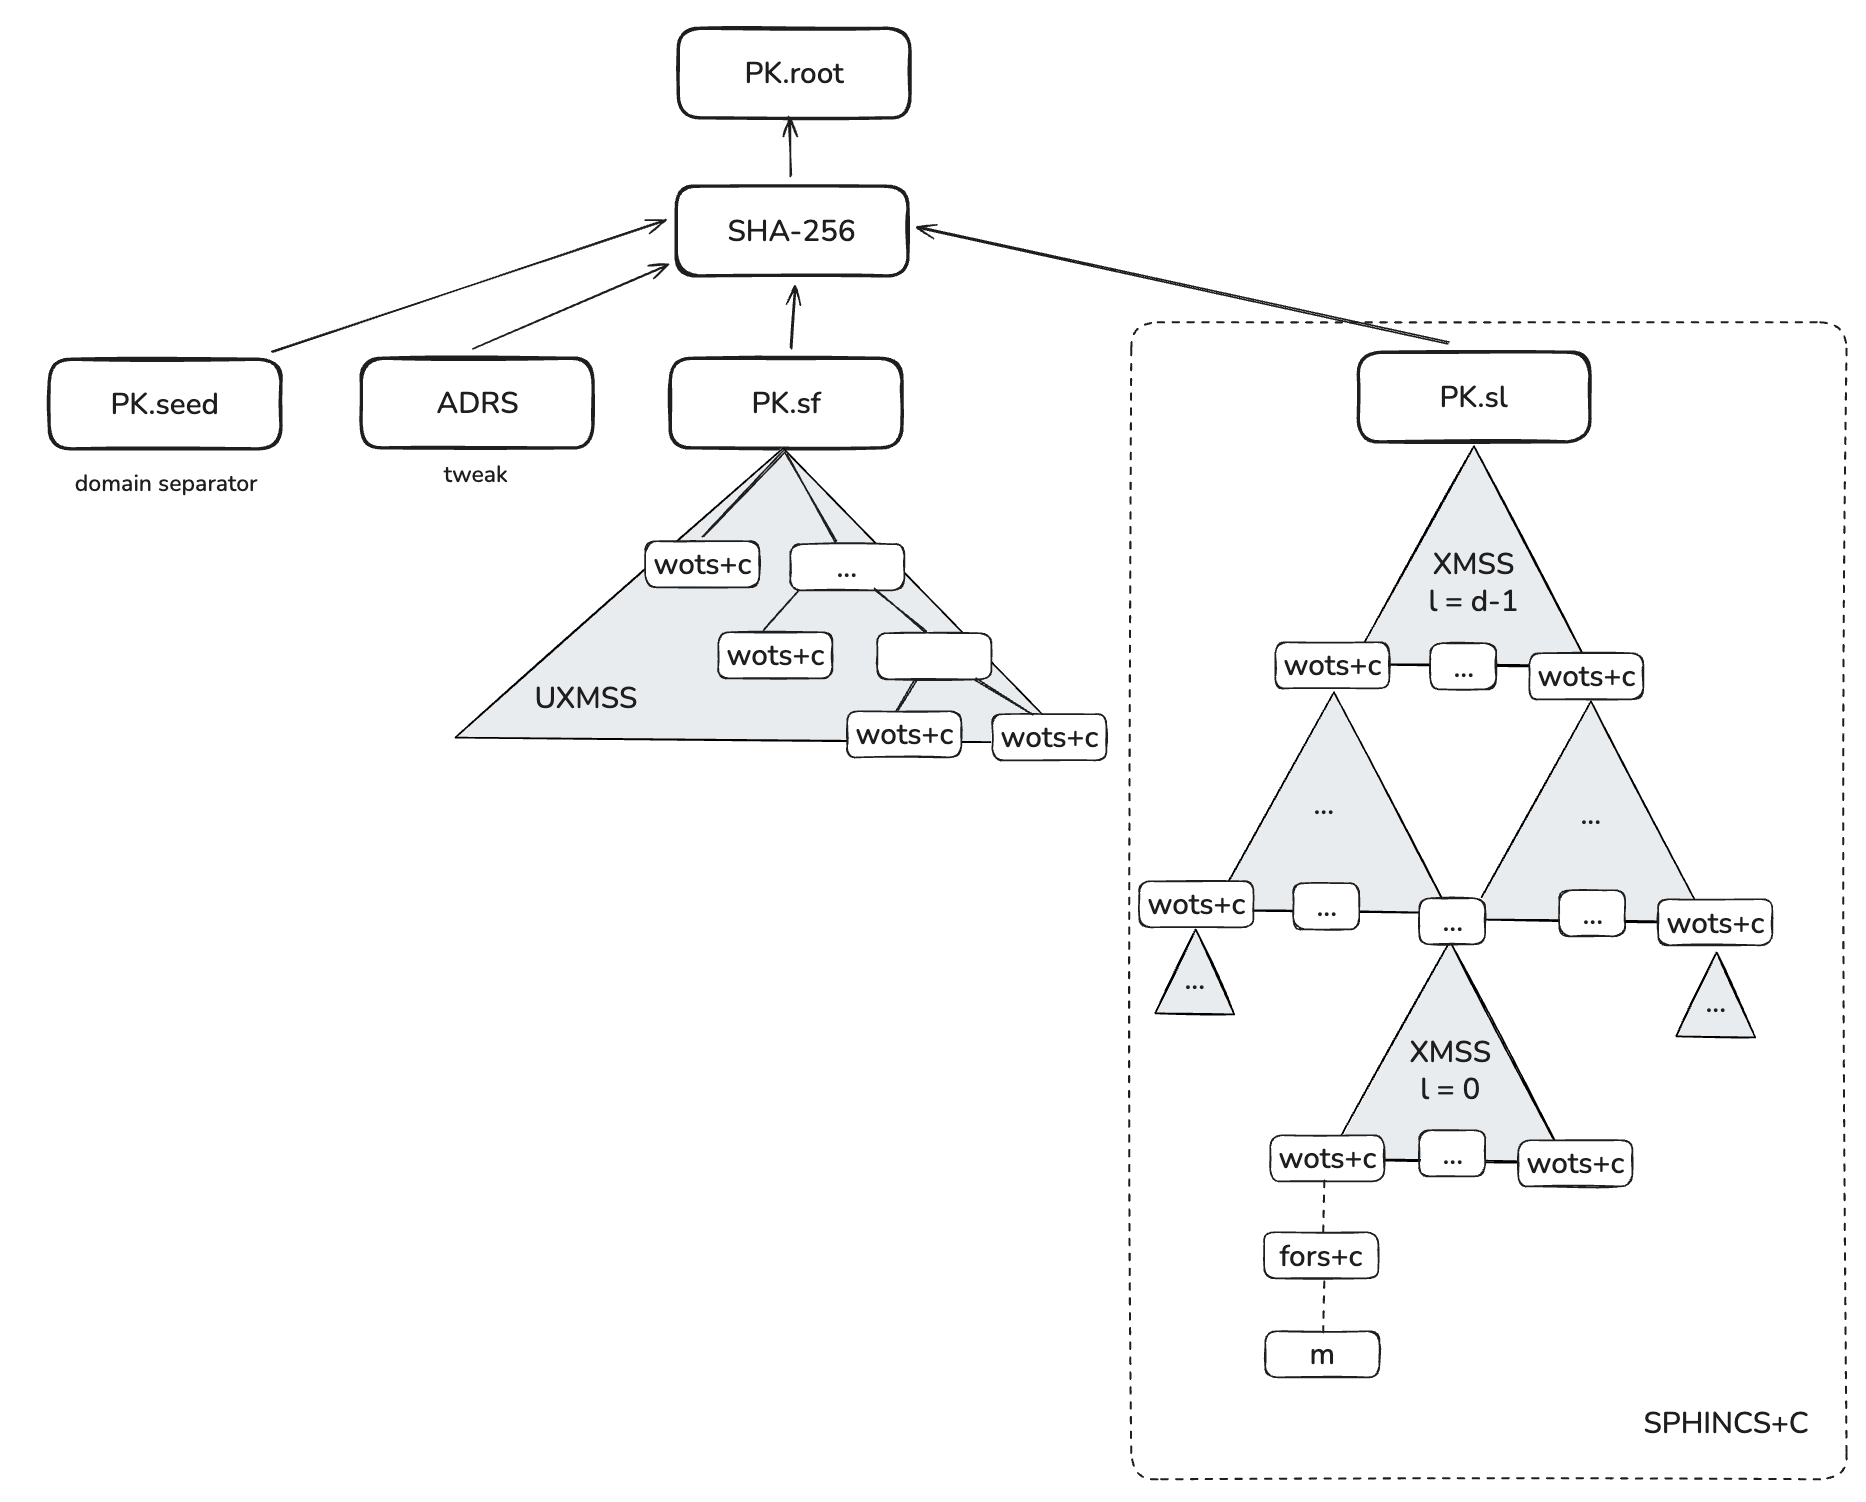
\includegraphics[width=1\linewidth]{content/img/general.png}
    \caption{SHRINCS architecture}
    \label{fig:shrincs}
\end{figure}

\subsection{Key Pair Derivation and Size}
SHRINCS keys are derived from a single random seed:
\begin{verbatim}
    seed ←$ {0,1}^(3*8*n)   // 3n bytes
\end{verbatim}
Seed allows to derive a private key \texttt{SK ← (SK.seed, SK.prf, PK.seed, PK.sf, PK.sl, PK.root)}:
\begin{verbatim}
    SK.seed ← seed[0:n]     // Seed for key derivation
    SK.prf ← seed[n:2n]     // Secret needed for PRF_msg
    PK.seed ← seed[2n:3n]   // Domain separator for different SHRINCS key pairs
    PK.sf ← compute_stateful_root(PK.seed, ADRS, SK.seed) // Public stateful key
    PK.sl ← compute_stateless_root(PK.seed, ADRS, SK.seed) // Public stateless key
    PK.root ← H(PK.seed, ADRS, PK.sf, PK.sl) // Root public key
\end{verbatim}
where \texttt{ADRS} is a tweak also known as a context address (see Section~5.5). \\

The size of the secret key is \texttt{6n} bytes. A public key consists of two values \texttt{PK ← (PK.seed, PK.root)} and has a size of \texttt{2n} bytes.

\subsection{Signature Size and Verification Cost}
We have different methods to calculate signature size and verification cost based on the used mode. 
\subsubsection{Stateful}
Stateful signatures consist of:
\begin{enumerate}
    \item \texttt{PK.sl}: the stateless public key (for unified verification)
    \item \texttt{R}: randomness for message hashing (with the size \texttt{R\_SIZE})
    \item \texttt{ctr}: grinding counter of the size \texttt{c}
    \item \texttt{chain\_values}: WOTS+C signature (\texttt{l} chains)
    \item \texttt{auth\_path}: UXMSS authentication path (\texttt{min(q, hsf)} nodes)
\end{enumerate}

Signature size calculation: 
\begin{verbatim}
    General formula: size = PK.sl_SIZE + R_SIZE + c + l*n + min(q, hsf)*n 
           SHRINCS-B.size = 16 + 32 + 4 + 16*16 + q*16              = 308 + 16q
           SHRINCS-L.size = 16 + 32 + 4 + 64*16 + q*16              = 1076 + 16q
\end{verbatim}

The signature verification cost is:
\begin{verbatim}
    General formula: hash_ops = (w-1)*l - S_wn + min(q, hsf) + 2 
           SHRINCS-B.hash_ops = 255*16 - 2040 + q + 2               = 2042 + q
           SHRINCS-L.hash_ops = 3*64 - 140  + q + 2                 = 54 + q
\end{verbatim}

\paragraph{Note:} \texttt{w} is the Winternitz parameter and \texttt{S\_wn} is a target grinding value for WOTS+C instance (see Section~6). Two additional hashes include: (1) the hash to receive a compressed WOTS+C key; (2) the hash to obtain the root public key.

\subsubsection{Stateless}
Stateless signatures consist of:
\begin{enumerate}
    \item \texttt{PK.sf}: the stateful public key (unified verification)
    \item FORS+C signature: few-time signature on the message
    \item HT signature: \texttt{d} XMSS signatures forming the hypertree
\end{enumerate}

Signature size calculation: 
\begin{verbatim}
    General formula: size = PK.sf_SIZE + fors_size(R_SIZE + (k-1)*(n + a*n))
                      + xmss_layer_size(R_SIZE + c + l*n + h'*n) * d

    SHRINCS-B.size = 16 + fors_size(32 + 5*(16 + 22*16))
                    + xmss_layer_size(32 + 4 + 16*16 + 12*16) * 2
                    = 16 + (32 + 1840) + (32 + 4 + 256 + 192) * 2
                    = 16 + 1872 + 968 = 2856

    SHRINCS-L.size = 16 + fors_size(32 + 5*(16 + 22*16))
                    + xmss_layer_size(32 + 4 + 64*16 + 12*16) * 2
                    = 16 + (32 + 1840) + (32 + 4 + 1024 + 192) * 2
                    = 16 + 1872 + 2504 = 4392
\end{verbatim}

The signature verification cost is:
\begin{verbatim}
    General formula:
        fors_hashes = (k-1)*(1 + a) + 1
        wots_per_layer = (w-1)*l - S_wn + 1
        xmss_per_layer = wots_per_layer + h'
        total = fors_hashes + d*xmss_per_layer + 1

    SHRINCS-B:
        fors_hashes = 5*23 + 1 = 116
        wots_per_layer = (256-1)*16 - 2040 + 1 = 2041
        xmss_per_layer = 2041 + 12 = 2053
        total = 116 + 2*2053 + 1 = 4223 hashes

    SHRINCS-L:
        fors_hashes = 116
        wots_per_layer = (w-1)*l - S_wn + 1 = 53
        xmss_per_layer = wots_per_layer + h' = 53 + 12 = 65
        total = fors_hashes + d*xmss_per_layer + 1
              = 116 + 2*65 + 1 = 247 hashes
\end{verbatim}

\paragraph{Note:} \texttt{k} (number of trees) and \texttt{a} (tree height) are parameters of FORS+ (see Section~9). \texttt{h'} is the height of internal tree in HT. One additional hash is required to obtain the root public key after stateless public key recovery. 